\chapter{Measuring the Helicity Polarisation of the $\PW$ Boson}
\section{Introduction}
The study of \Wjets production at a hadron collider presents an important
opportunity for furthering understanding of the underlying Electroweak and
\ac{QCD} processes. In particular, since it is one of a relatively small number
of processes for which highly precise \ac{NLO} calculations have been performed,
experimental measurements can give a direct constraint on the \acp{PDF}. \Wjets
production is also of considerable interest in the context of \ac{NP} searches
where these events are often a dominant background. Finally, the neutrino in the
leptonic decay mode provides a source of ``real'' missing energy which can be
useful in the understanding of detector effects relevant to searches for
\acs{WIMP}-type particles present in \ac{SUSY} and other theories.

\section{Background}
Some theoretical background relating to \PW helicity effects has been presented
in Section~TODO. Here, the discussion will be oriented towards a more
experimental context.

\subsection{Polarisation Effects Parallel to the Beam Line}
For small values of \PW transverse momentum, \PtW the differential angular
cross-section for the process
$\Pp\Pp\longrightarrow\PWpm\longrightarrow\Plpm\Pgnl$ follows the Drell-Yan
distribution
\begin{equation}
\frac{dN}{d(\cos\theta)} \propto (1\mp \cos\theta)^2
\end{equation}

It is well known from straightforward helicity arguments\cite{mirkes_w_1994}that
\PW produced along the beam axis will exhibit a 100\% left-handed polarization. This
can be seen by considering the leading order partonic subprocesses
\begin{equation}
\Pup\APdown \longrightarrow \PWp \qquad\textrm{and}\qquad
\Pdown\APup\longrightarrow\PWm
\end{equation}
Firstly, note that the fraction of the proton momentum carried by the quark (as
determined by the \aclp{PDF}) is greater than that of the anti-quark. In
addition given that the \ac{LHC} is a $\Pp\Pp$ collider, valence anti-quarks are
not present. Anti-quarks must be drawn from the sea and are therefore likely to
be low momentum. Taking these two facts together, the quark is very likely to be
higher momentum than the anti-quark. By momentum conservation, it is expected
that the \PW will be produced overwhelmingly in the direction of the original
quark. Then given the \VminusA nature of the weak interaction, it is seen that
the quark must be left-handed and, by helicity conservation the \PW will be
polarised nearly 100\% left-handedly along the beam axis. A small dilution will
occur in instances where the anti-quark has by chance a larger momentum fraction
than the quark.

It is worth mentioning that the situation is not identical at the Tevatron
$\Pp\Pap$ collider. Although the \PWp also possess a 100\% left-handed
polarisation along the beamline (via similar arguments to those given above),
the \PWm are found to have a near 100\% right-handed polarisation. This is a
result of the subprocess $\APup\Pdown\longrightarrow\PWm$ where this time the
\APup carries more momentum.

% TODO: Mention the effect this has on the rapidity distribution

\subsection{Polarisation Effects in the Transverse Plane}
\label{sec:polarisation}
In the case, where the \PW carries a significant transverse momentum \PtW, the
situation is more complex. In general, the \PW may be produced in association
with a number of jets. For the sake of this discussion we will consider cases
involving only a single jet. Also, in order to simplify matters, one only needs
to consider the \PWp case as the \PWm case is very similar. At leading order,
three subprocesses should be considered\cite{berger_left_handed_w},
\begin{equation}
\Pup\Pgluon\longrightarrow\PWp\Pdown\;\textrm{,} \qquad
\Pup\APdown\longrightarrow\PWp\Pgluon\qquad\textrm{and} \qquad
\Pgluon\APdown\longrightarrow\PWp\APup
\label{eqn:w1jet_processes}
\end{equation}
For sufficiently large \PtW, the soft gluon enhancement of
$\Pup\APdown\longrightarrow\PWp\Pgluon$ and the quark-gluon subprocess is found
to dominate. It has been found that 70-80\% of $\PW+N$~jet ($N \leq 4$)
production at \ac{LO} is initiated by this subprocess.

Considering the quark-gluon subprocess, the $s$ and $t$ channel diagrams are
shown in Figure~\ref{fig:w1jet_st}. For the $s$ channel diagram, the on-shell
\Pdown quark is directly coupled to the \PW and therefore must be in a negative
helicity state (i.e. left-handed). Assuming a positive helicity for the W boson
(as depicted in Figure~\ref{fig:w1jet_st_s}), the spin along the $\PW\Pdown$
axis is $1+\frac{1}{2} = \frac{3}{2}$. Such a configuration is not allowed for the
\spinhalf off-shell quark and thus the $s$-channel diagram should lead to a 100\%
left-handed polarisation of the \PW. In contrast, the $t$ channel diagram is not
similarly constrained by spin arguments (since the \PW is not coupled directly
to the quark) and thus the helicity polarisation will not be seen.

It can be shown that for a left-handed incoming gluon, the $t$-channel diagram
can be made to vanish. For a right-handed gluon, the \PW polarisation is not
constrained but has been shown to become predominantly right-handed at high
\PtW. At high \PtW, the outgoing \PW helicity will be almost 100\% correlated
with the incoming gluon and due to a factor 4 difference in the size of the
corresponding matrix elements, the \PW is expected to asymptotically approach an
80\% left-handed polarisation with increasing \PtW. Due to the \VminusA
coupling, the decay leptons may act as an analyser of the \PW
polarisation. Having provided some motivation for the existence of the effect, a
more detailed discussion will follow.

\begin{figure}
\centering
\subfloat[]{\label{fig:w1jet_st_s}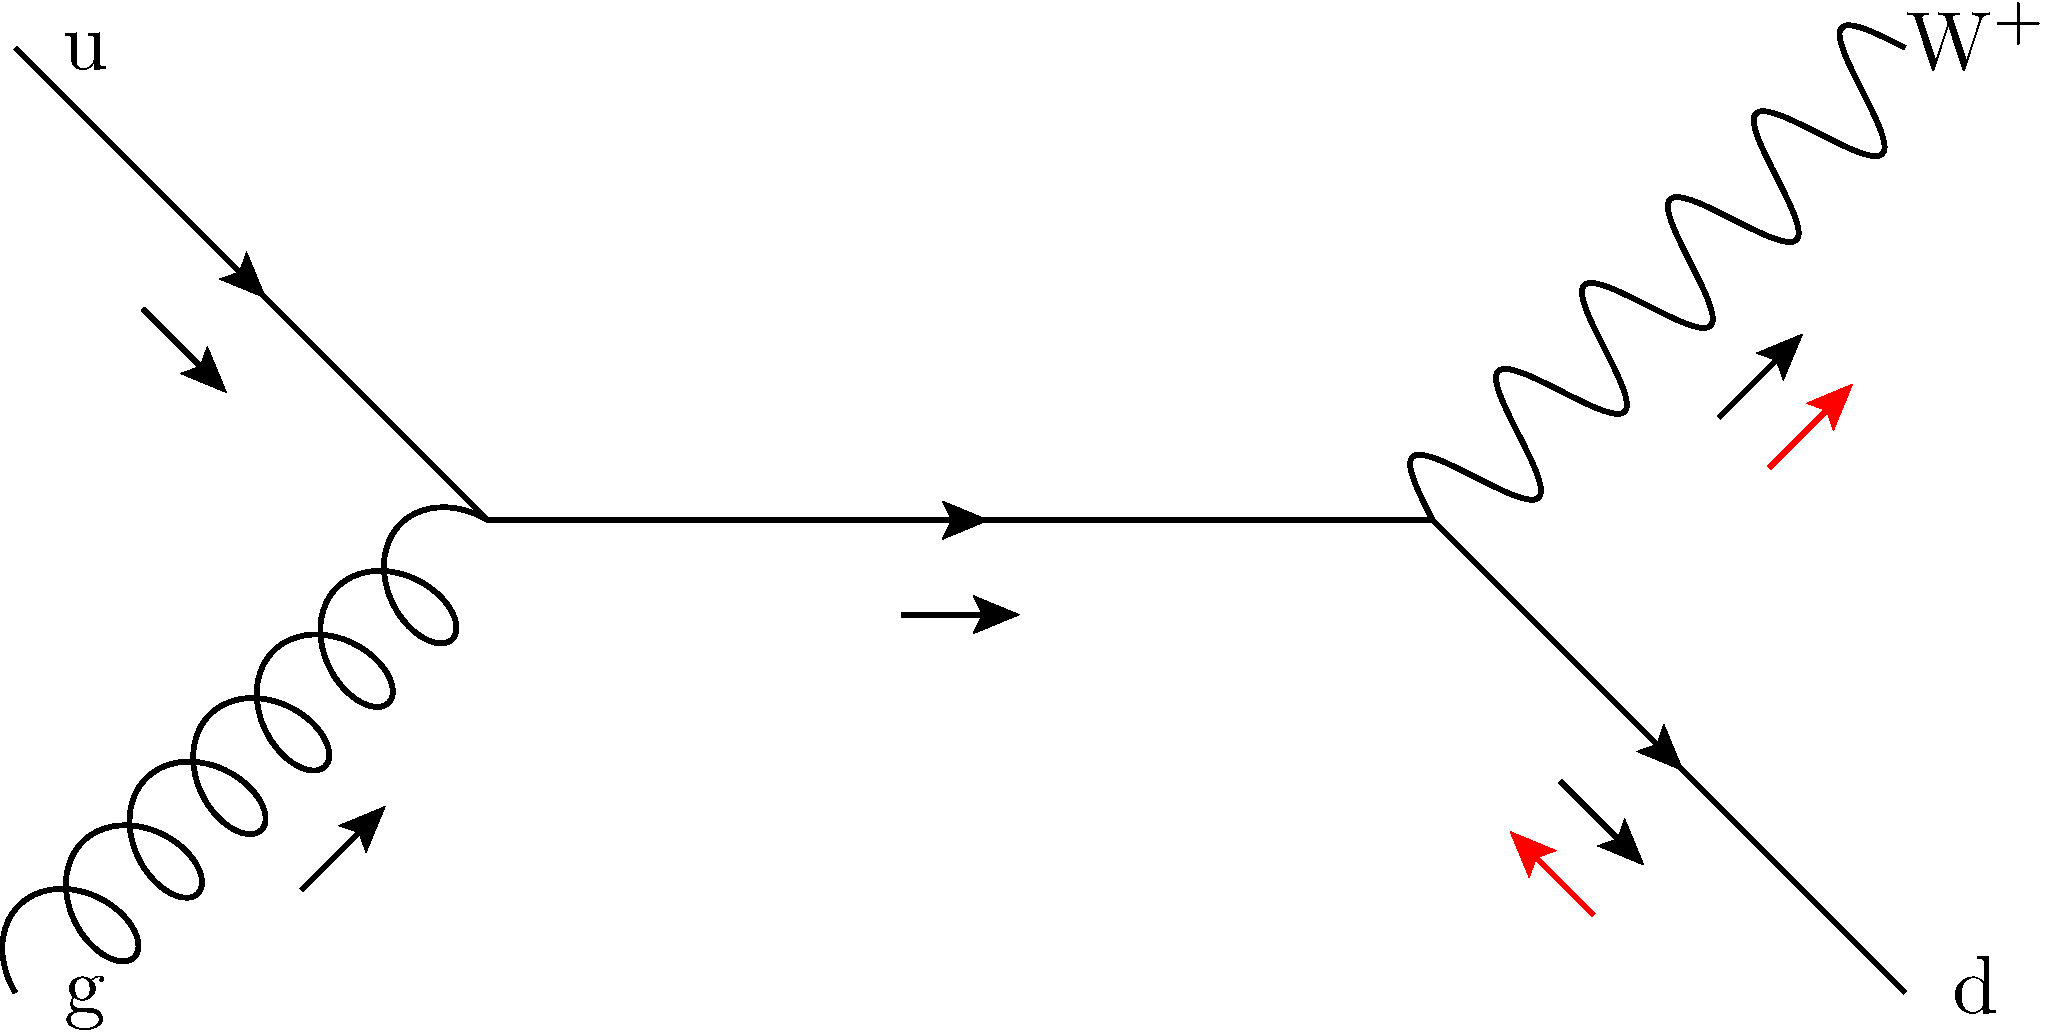
\includegraphics[width=0.5\textwidth]{fig/wpol_1jet_s}}\quad
\subfloat[]{\label{fig:w1jet_st_t}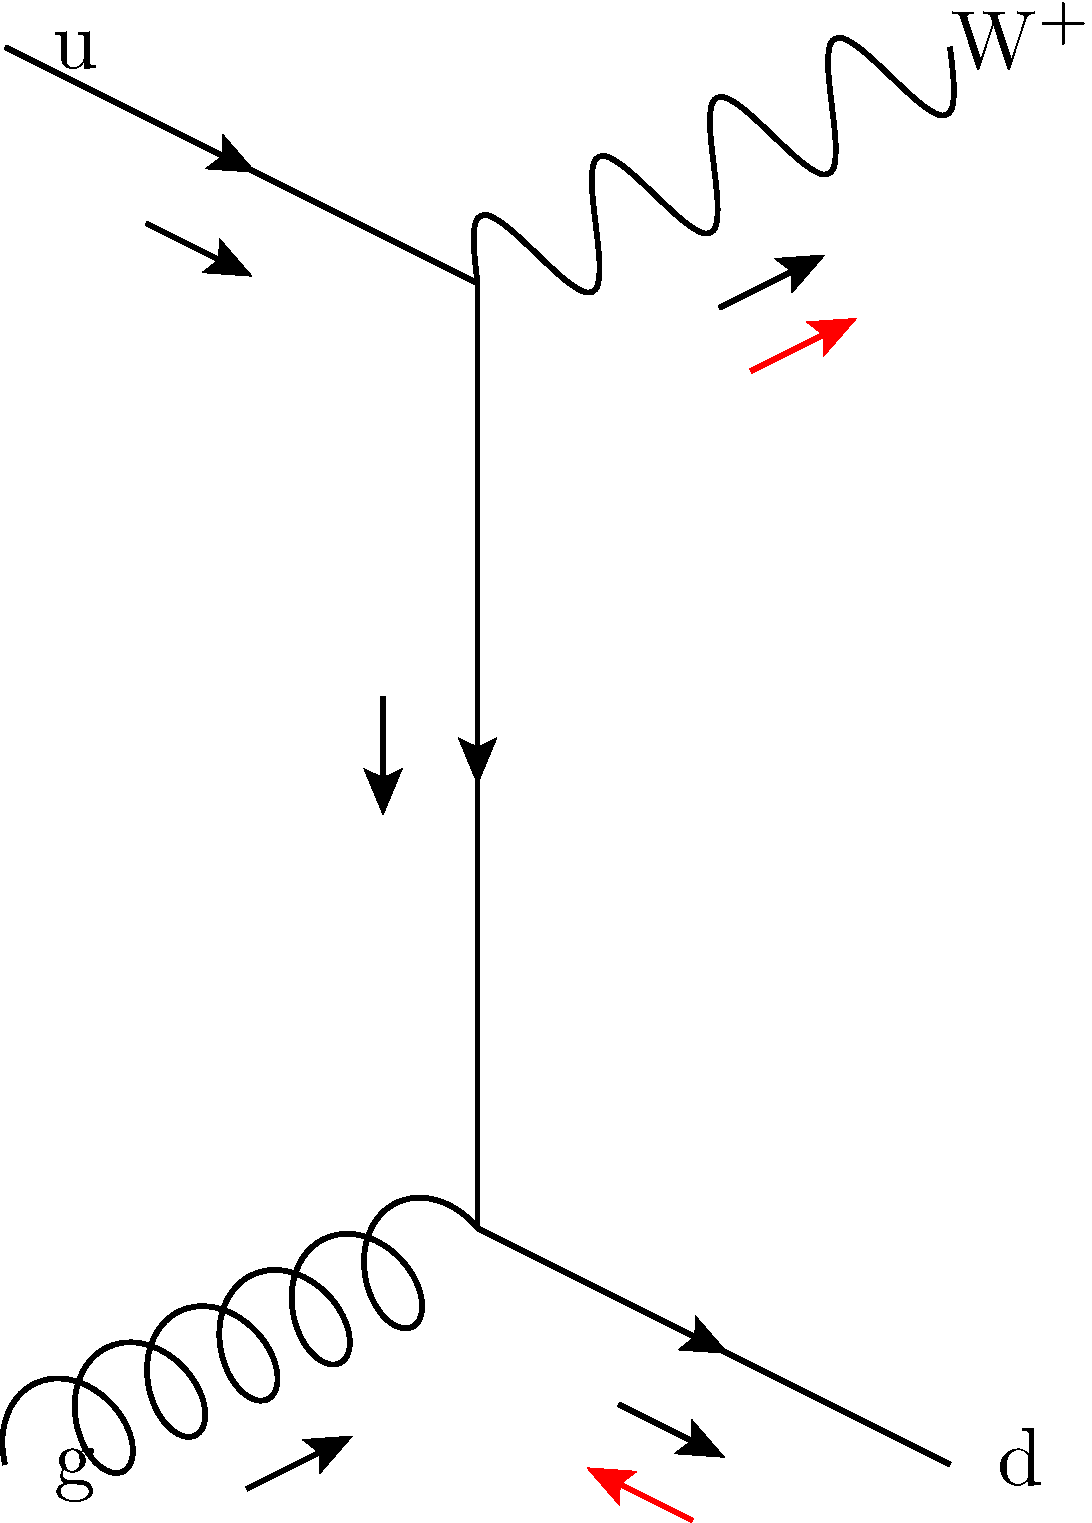
\includegraphics[width=0.25\textwidth]{fig/wpol_1jet_t}}
\caption{Diagrams showing the $\Pup\Pgluon\longrightarrow\PWp\Pdown$ subprocess
  in the \subref{fig:w1jet_st_s} $s$ and \subref{fig:w1jet_st_t} $t$ channels. The black displaced arrows indicate the particle
  momenta. For the $s$ channel diagram, the helicity vectors are shown as red
  arrows, for the case of a right-handed \PW boson.}
\label{fig:w1jet_st}
\end{figure}

Writing the amplitudes of the subprocesses in Equation~\ref{eqn:w1jet_processes}
in terms of spinor products, two distinct expressions emerge,

\begin{eqnarray*}
\mathcal{A}^{\textrm{tree}}_{(a)} &\propto&
\frac{\left<\Pdown\nu\right>^2}{\left<\Pup\Pgluon\right>\left<\Pgluon\Pdown\right>}\\
\mathcal{A}^{\textrm{tree}}_{(b)} &\propto&
\frac{\left[\Pup\Pe\right]^2}{\left[\Pup\Pgluon\right]\left[\Pgluon\Pdown\right]}
\end{eqnarray*}
where factors common to both expressions are not shown. The corresponding
cross-sections are
\begin{equation}
d\sigma^{\textrm{LO}}_{(a)} \propto (k_{\Pdown} \dot k_{\Pneutrino})^2 \quad
d\sigma^{\textrm{LO}}_{(b)} \propto (k_{\Pup} \dot k_{\Pe})^2
\label{eqn:w1jet_xs}
\end{equation}
where the $k$ are Lorentz vectors representing the particle momenta. For each
subprocess, the helicity configurations corresponding to $(a)$ and $(b)$ are
shown in the upper and lower rows of Figure~\ref{fig:w1jet_modes}
respectively. The red arrows indicate particle helicity, with a double-stemmed
arrow for the \PW momentum. In the cases where the \PW is neither purely
left-handed nor right-handed, the arrow is placed at an angle.

Starting with the subprocess $\Pup\Pgluon\longrightarrow\PWp\Pdown$, the $(a)$
expression in \ref{eqn:w1jet_xs} correlates the axis of the \Pdown quark with the
neutrino (see Figure~\ref{fig:w1jet_modes_1a}). Due to the \VminusA coupling, the
neutrino must have a left-handed helicity and, via angular momentum
conservation, so too the \PW. The angular dependence is
$(1-\cos\tilde{\theta}^*)^2$ where $\tilde{\theta^*}$ is the angle of the
charged decay lepton with the \PW flight direction in the centre of mass
frame. In contrast, considering an identical particle configuration but with
helicities corresponding to $(b)$ (Figure~\ref{fig:w1jet_modes_1b}), the
\Ppositron direction is now correlated with the incoming beam
direction. Boosting to the \PW rest frame, at high \PtW, the incoming quark and
gluon are nearly parallel and, given a scattering angle of 90\degrees, the \Pup
quark momentum is seen to be half that of the \Pdown quark. The angular
dependence is thus $\frac{1}{4}(1+\cos\tilde{\theta}^*)^2$ yielding a
right-handed polarisation at a quarter of the rate of the left-handed component.

For the subdominant process $\Pup\APdown\longrightarrow\PWp\Pgluon$, the terms
in Eqn~\ref{eqn:w1jet_xs} correlate the momenta of the decay leptons with the
beam direction. The two cases are shown in Figures~\ref{fig:w1jet_modes_2a} and
\ref{fig:w1jet_modes_2b}. Although it can be seen once again that a left-handed
and right-handed polarisation emerge, in this case they are found to cancel for
a scattering angle of 90\degrees and thus give no net polarisation. Lastly, for
the subprocess $\Pgluon\APdown\longrightarrow\PWp\APup$, show in
Figures~\ref{fig:w1jet_modes_3a} and \ref{fig:w1jet_modes_3b}, the $(b)$
contribution correlated the \Pup quark with the \Ppositron direction, leading to a
dominantly right-handed polarisation. However, since the \ac{PDF} $\APdown(x)$
is much smaller than $\Pup(x)$, this effect is largely washed out by the
dominant left-handed polarisation mode.

\begin{figure}
\centering
\subfloat[]{\label{fig:w1jet_modes_1a}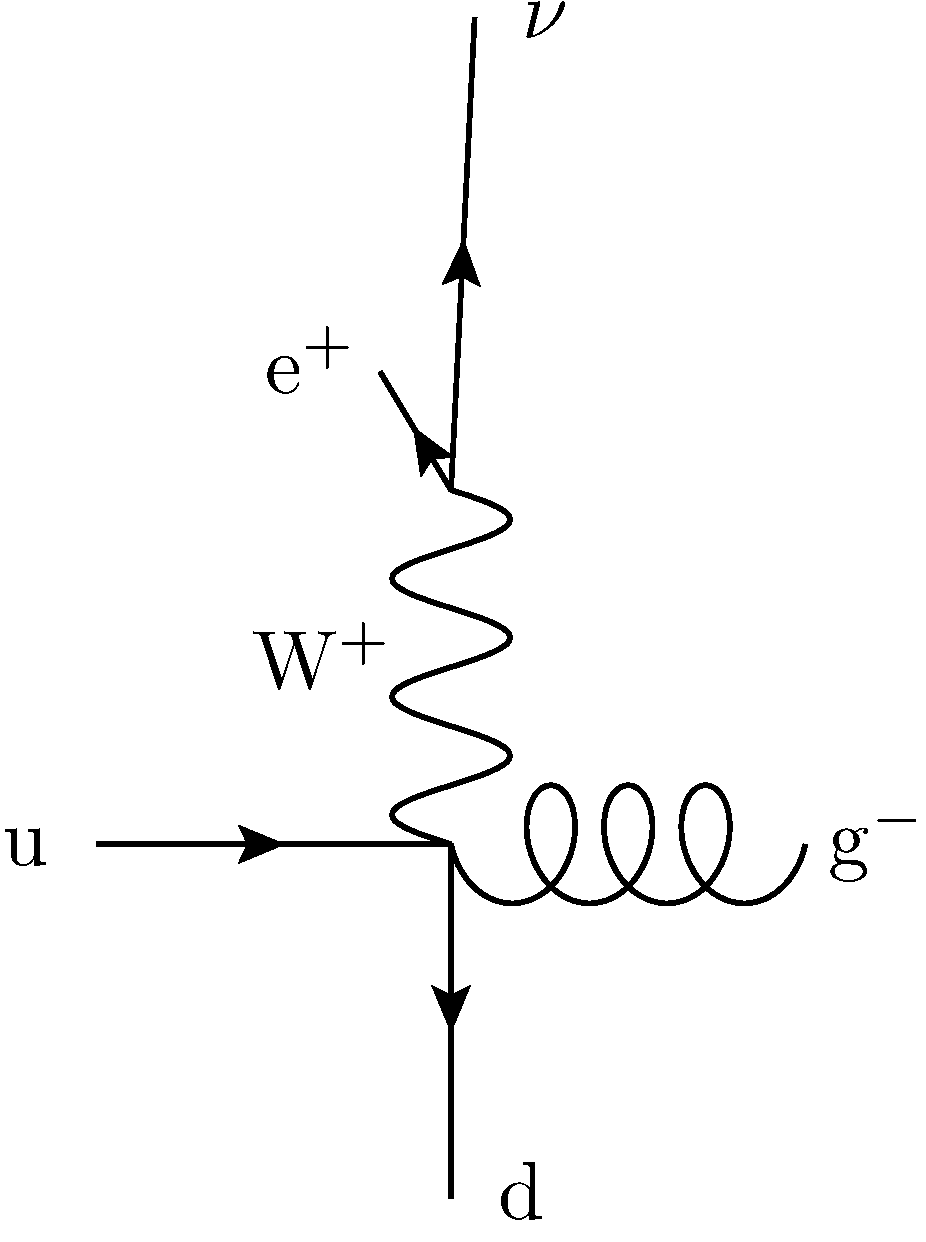
\includegraphics[width=0.3\textwidth]{fig/wpol_prod_a}}\quad
\subfloat[]{\label{fig:w1jet_modes_2a}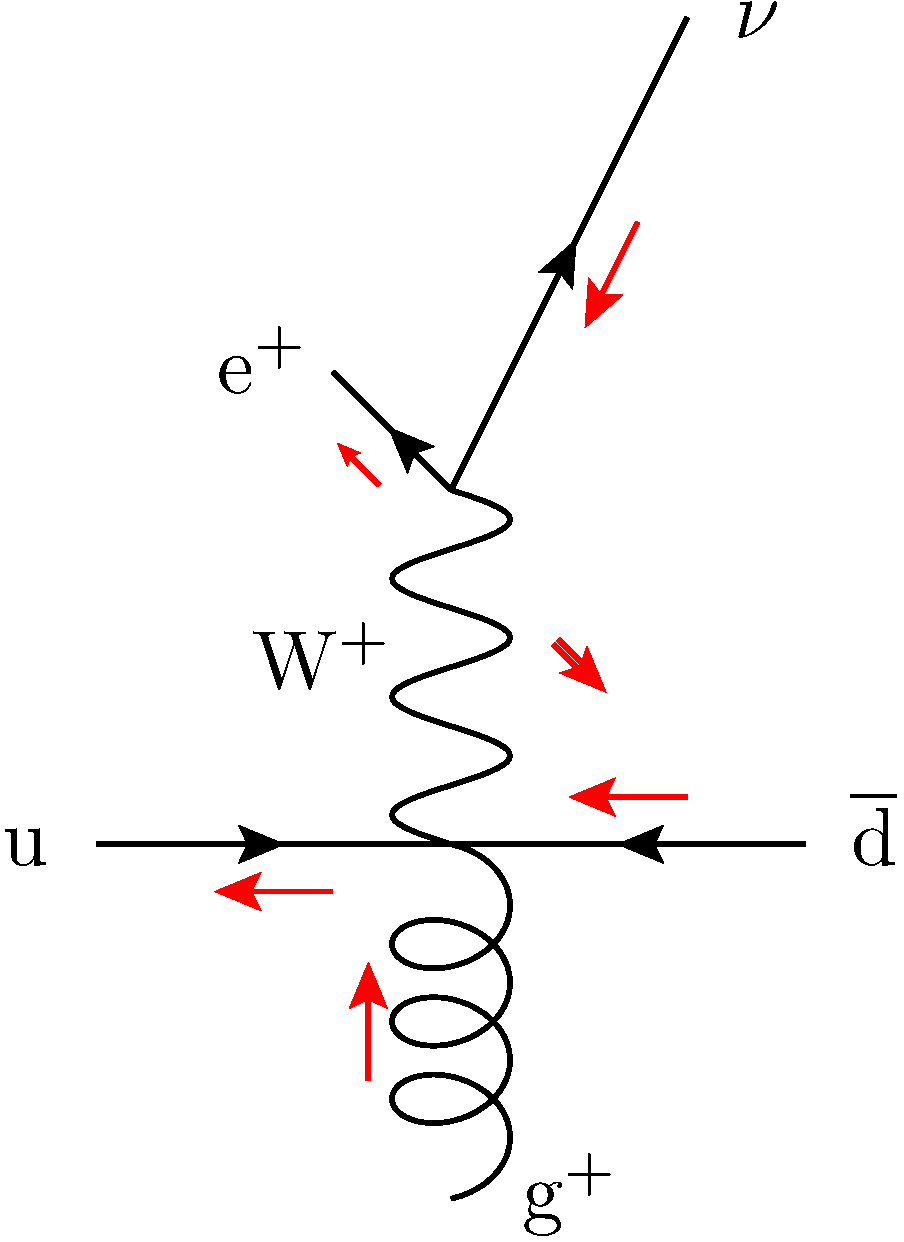
\includegraphics[width=0.3\textwidth]{fig/wpol_prod_b}}\quad
\subfloat[]{\label{fig:w1jet_modes_3a}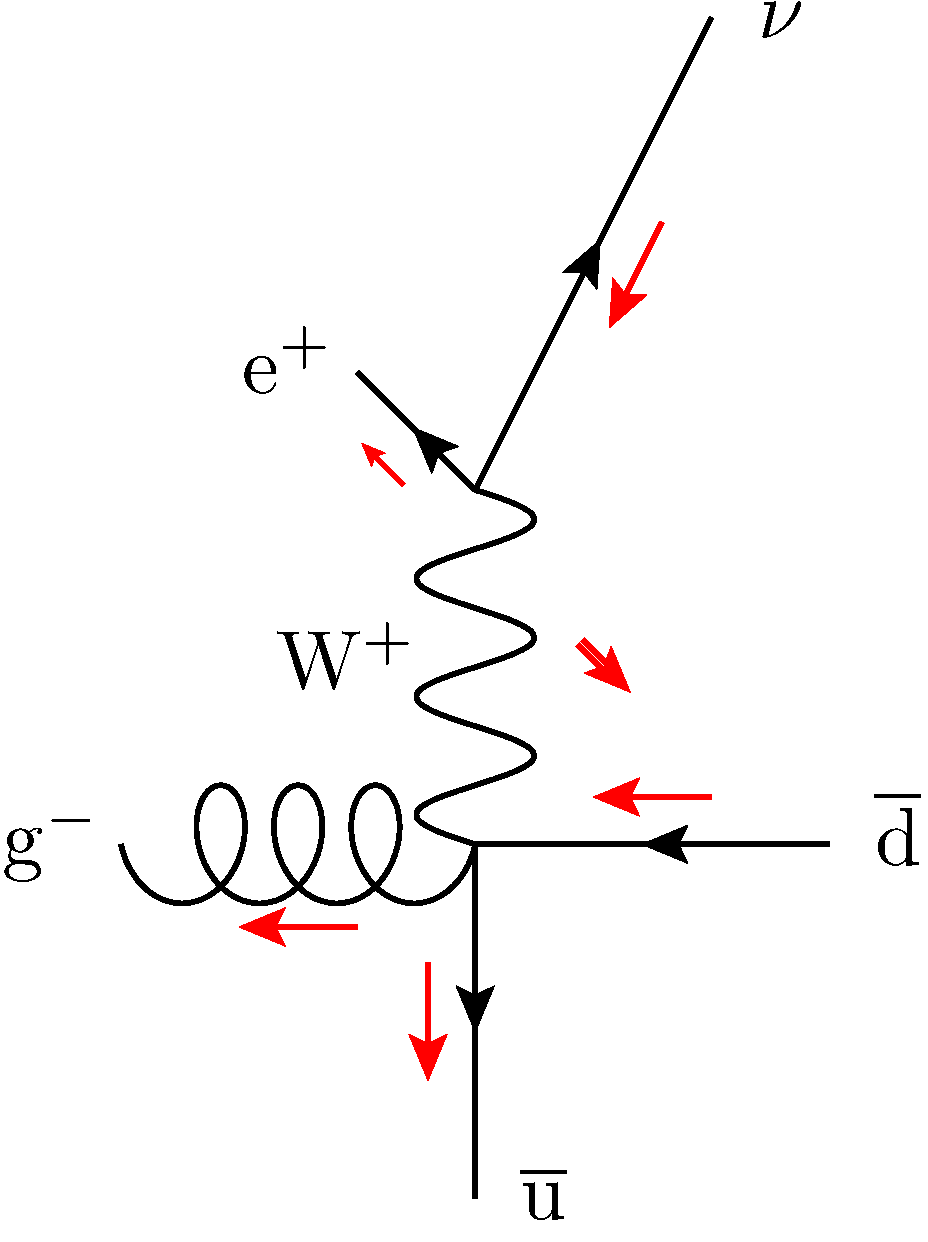
\includegraphics[width=0.3\textwidth]{fig/wpol_prod_c}}\\
\subfloat[]{\label{fig:w1jet_modes_1b}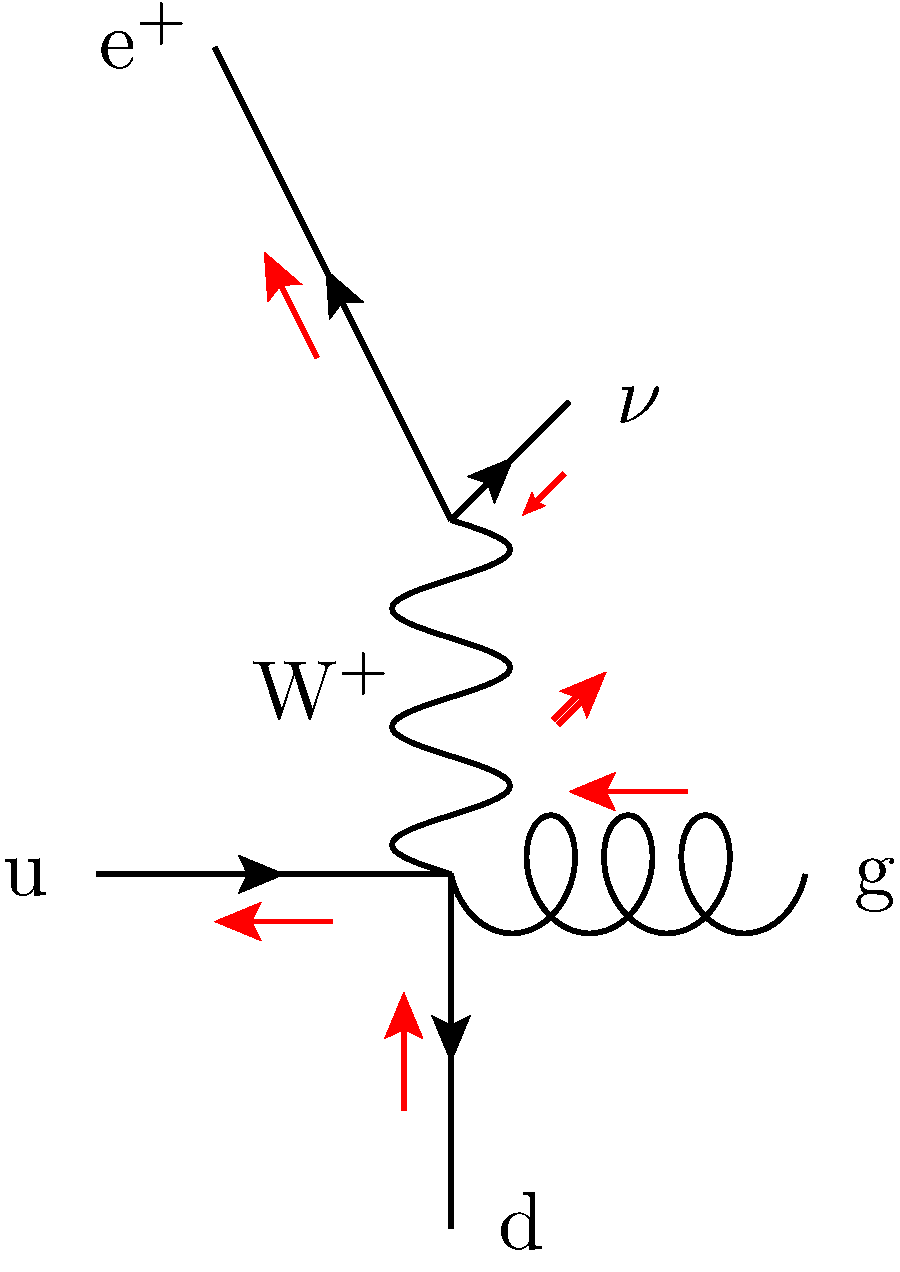
\includegraphics[width=0.3\textwidth]{fig/wpol_prod_d}}\quad
\subfloat[]{\label{fig:w1jet_modes_2b}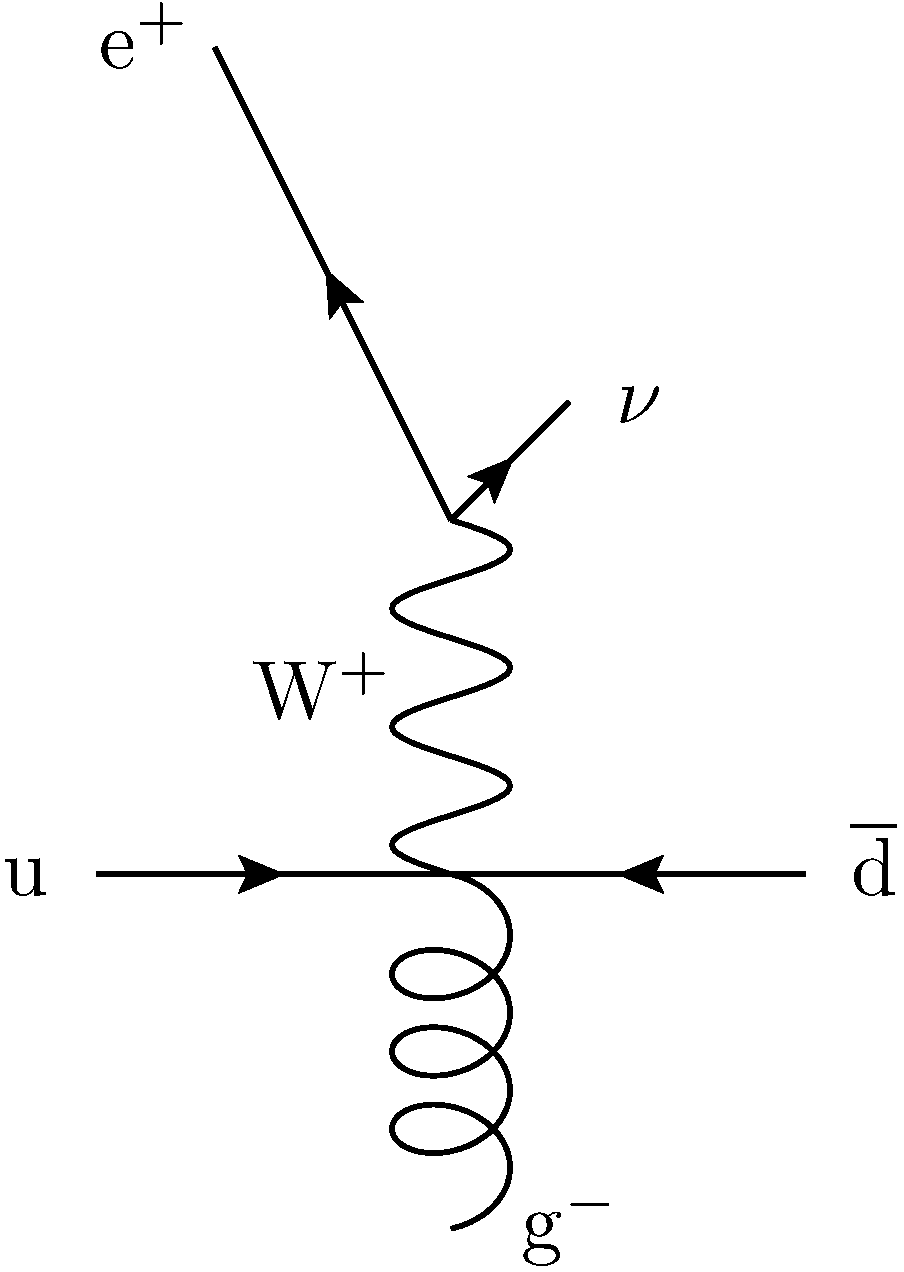
\includegraphics[width=0.3\textwidth]{fig/wpol_prod_e}}\quad
\subfloat[]{\label{fig:w1jet_modes_3b}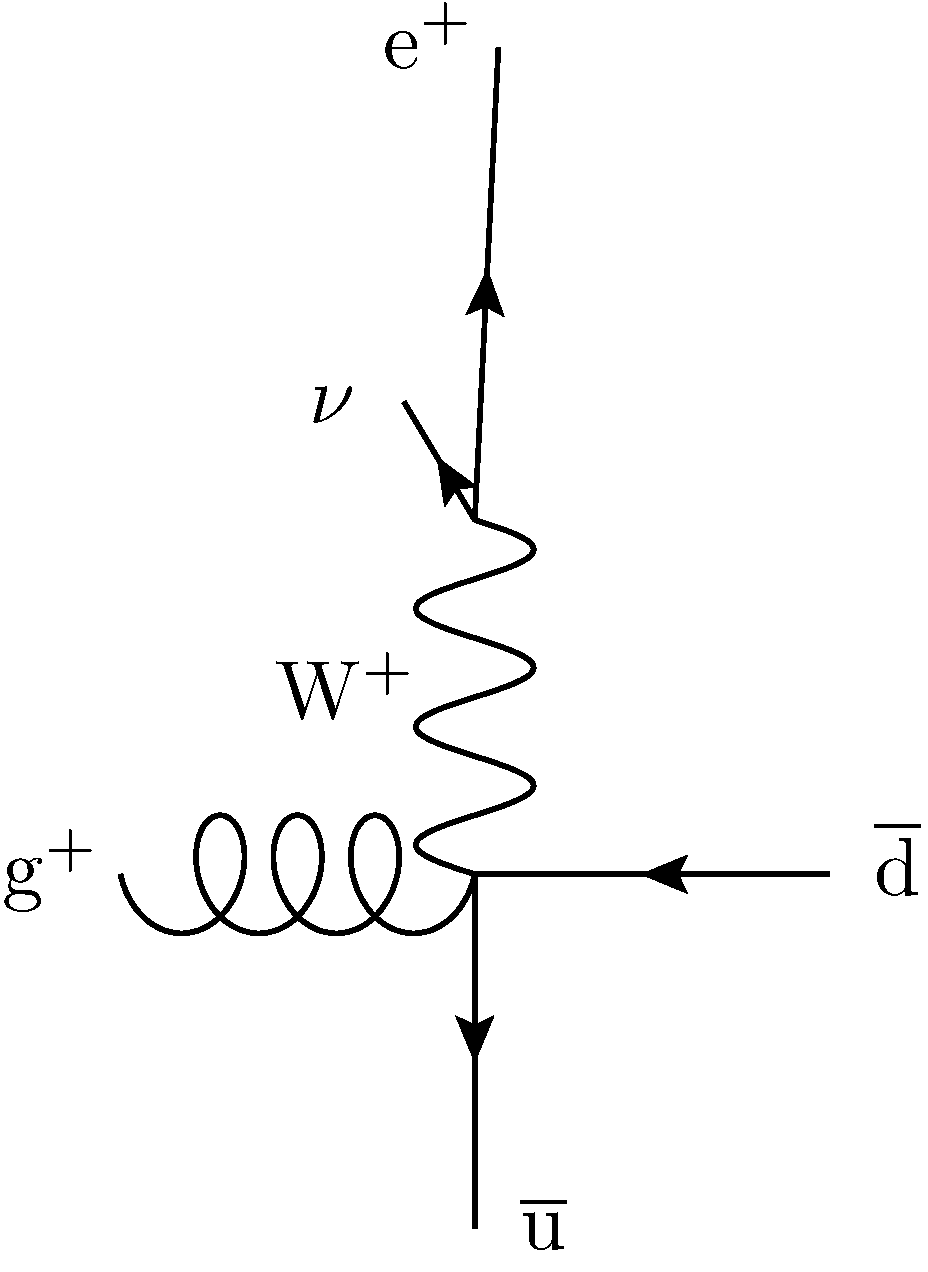
\includegraphics[width=0.3\textwidth]{fig/wpol_prod_f}}
\caption{Illustrations of $\PWplus+1$~jet production modes at the LHC. The
  gluon superscript indicates its helicity}
\label{fig:w1jet_modes}
\end{figure}


\subsection{Studying Helicity}

\subsubsection{The Helicity Frame}
The polarisation effects may be conveniently studied within the helicity frame
of the \PW boson. This is defined as the rest frame of the \PW with the
polarisation axis (here, the z-axis) is aligned along the line of flight of the
\PW in the lab frame. The x-axis is then chosen to lie along the plane spanned
by the two colliding protons in the boson rest frame with the sense chosen such
that the angle between it and the nearest proton is minimised. The y-axis is
then fixed to be perpendicular to these two. The polar angle, \thetastar is
measured in the $y-z$ plane between the positive z-axis and the
lepton. Likewise, the azimuthal angle, \phistar is measured in $x-z$ between the
positive $x$ axis and the lepton. This arrangement is illustrated in
Figure~\ref{fig:wpol_helicity_frame}. For $0 < |\phistar| < \frac{\pi}{2}$, the
charged lepton will have a larger rapidity that the \PW boson and thus a smaller
\Pt. Alternatively, for $\frac{\pi}{2} < |\phistar| < \pi$, the lepton
will have a smaller rapidity and a larger \Pt.

\begin{figure}
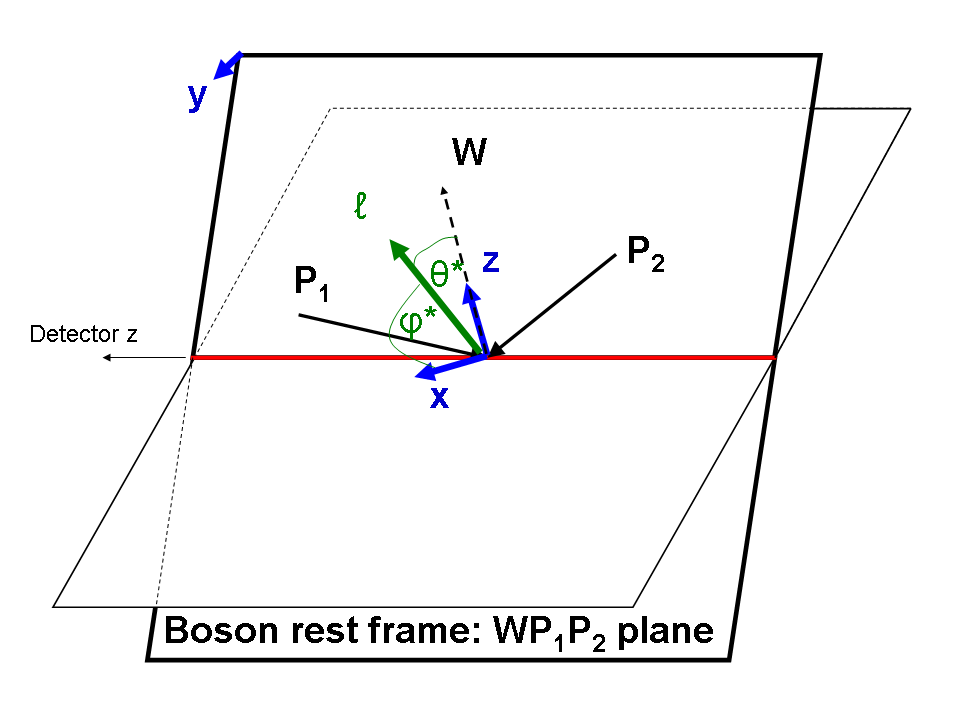
\includegraphics[width=0.8\textwidth]{fig/helicity_frame_polnote}
\caption{The Helicity Frame}
\label{fig:wpol_helicity_frame}
\end{figure}

\subsubsection{Quantifying Helicity}
The hadronic cross-section of the \PW is obtained within the parton model by
weighting the individual parton-level cross-sections by the respective parton
densities \cite{mirkes_w_1994},
\begin{equation}
\frac{d\sigma^{h_1 h_2}}{d(\PtW)^2 dy d\Omega^*} = \sum_{ab} \int dx_1 dx_2
f_a^{h_1}\left(x_1, \mu_F^2\right)f_b^{h_2}\left(x_2, \mu_F^2\right)
\times \frac{s d\tilde{\sigma}_{ab}}{dt du d\Omega^*} \left(x_1 P_1, x_2 P_2,
\alpha_s (\mu_R^2)\right)
\end{equation}
where $h_1$ and $h_2$ are the interacting hadrons and the sum runs over $a,b =
\Pquark, \APquark, \Pgluon$. The parton density functions $f_a^{h}\left(x,
  \mu^2\right)$ give the probability of finding a parton $a$ with momentum
fraction $x$ in hadron $h$ when probed at a scale $\mu^2$. The
$d\tilde{\sigma}_{ab}$ are the parton-level cross-sections for the chosen
process(es). The hadron-level Mandelstam variables are written uppercase
\begin{equation*}
S = (P_1 + P_2)^2 \qquad T = (P_1 - Q)^2 \qquad U = (P_2 - Q)^2
\end{equation*}
and parton-level lowercase
\begin{eqnarray*}
s &=& (p_1 + p_2)^2 = x_1 x_2 S\\
t &=& (p_1 - Q)^2  = x_1(T-Q)^2 +Q^2\\
u &=& (p_2 - Q)^2 = x_2(U -Q)^2 + Q^2
\end{eqnarray*}
and
\begin{equation*}
p_1 = x_1 P_1 \qquad p_2 = x_2 P_2
\end{equation*}
This can be rewritten in terms of a standard set of angular coefficient $A_i$,
to give\cite{mirkes_w_1992}
\begin{align}
\frac{d\sigma}{d(\PtW)^2 dy d\cos\theta d\phi} = \frac{3}{16\pi}
\frac{d\sigma^{-1}}{d(\PtW)^2 dy} &\left [ \left(1+\cos^2\theta\right) \right.\\
 &+ \frac{1}{2} A_0 \left ( 1 - 3\cos^2\theta \right ) + A_1 \sin 2\theta\cos\phi \\
 &+ \frac{1}{2}A_2\sin^2\theta\cos 2\phi + A_3\sin\theta\cos\phi \\
 &+ A_4\cos\theta + A_5\sin^2\theta\sin 2\phi \\
 &+ A_6\sin 2\theta\sin \phi + A_7\sin\theta\sin\phi
\label{eqn:wpol_diff_xs}
\end{align}

% TODO: Figure out the difference between  theta and theta*
The $A_i$ are ratios of the separate helicity cross-sections of the boson to its
total unpolarised cross-section and are dependent on the \PW boson charge,
transverse momentum \PtW and rapdidity \YW. Eqn~\ref{eqn:wpol_diff_xs} can be
integrated over $\phi$ and \PtW to give
\begin{equation}
\frac{d\sigma}{d\cos\theta} \propto \left(1+\cos^2\theta\right) +
\frac{1}{2}A_0\left(1-3\cos^2\theta\right) + A_4\cos\theta
\label{eqn:wpol_xs_Ai}
\end{equation}

% TODO: Check all this bs!
Due to the \VminusA nature of the Electroweak theory, the \PWp (\PWm) may couple
only to left-handed (right-handed) fermions and right-handed (left-handed)
anti-fermions, therefore the angular momentum state of the decay leptons is
\begin{eqnarray*}
\ket{\Pl\Pgn^{J,M}} &=& \ket{\frac{1}{2}, \pm \frac{1}{2}}
\oplus \ket{\frac{1}{2}, \pm\frac{1}{2}} \\
&=& \textrm{either}\quad\ket{1, +1}\quad\textrm{or}\quad \ket{1, -1}
\end{eqnarray*}
where $\ket{J, M}$ represents an angular momentum state with a total angular momentum $J$ and projection $M$.

Rotating these states through the angle \thetastar,
\begin{equation}
\ket{\Pl\Pgn^{J,M}}' = \sum_{M'=-J}^{M'=+J} d_{M, M'}^J \ket{J, M'}
\end{equation}
The angular momentum of a \PW boson in a helicity eigenstate is then
$\ket{\PW^{J,M''}}$. The matrix element for the angular momentum coupling can be
written
\begin{eqnarray*}
\braket{\PW^{J,M''}}{\Pl\Pgn^{J,M}}' &\sim& \sum_{M'=-J}^{M'=+J} d_{M M'}^{J}
\braket{J,M''}{J,M'} \\
&\sim& d^{J}_{M M''} \braket{J,M''}{J,M''} \sim d_{M M''}^{J}
\end{eqnarray*}
To calculate the cross-section, square the matrix elements and sum over the
helicity states ($M''$) of the incoming $\PW$, weighting each state by the helicity
fraction $f_{M''}$
\begin{equation}
\sigma(\PW\longrightarrow\Pl\Pgnl) \sim f_0 \left|d_{M 0}^1\right|^2 + f_{-1} \left|d_{M
    -1}^1\right|^2 + f_{1} \left|d_{M +1}^1\right|^2
\end{equation}
Where $f_0 + f_1 + f_{-1} = 1$. Finally, using the fact that for \PWpm, $M=\pm1$
and replacing for the elements of the D-matrices in terms of $\cos\thetastar$
\begin{equation}
\sigma(\thetastar_{\Plpm}) = \frac{\f0}{2}\sin^2\thetastar_{\Plpm} +
\frac{\fL}{4} \left(1\mp\cos\thetastar_{\Plpm}\right)^2 +
\frac{\fR}{4} \left(1\pm\cos\thetastar_{\Plpm}\right)^2
\label{eqn:wpol_helicity_fractions}
\end{equation}
Note that the helicity fractions $f_i$ have been relabelled to give a more
intuitive interpretation as the left-handed, right-handed and longitudinal
helicity fractions. Comparing now to Eqn~\ref{eqn:wpol_xs_Ai}, we identify $A_0
\sim f_0$ and $A_4 \sim \pm \fLmfR$. Whilst the $A_i$ are the more fundamental
parameters from a theoretical point of view, the helicity fractions \f0, \fL and
\fR are more readily interpreted in the context of the predictions of
Section~\ref{sec:polarisation}. In particular, at the LHC and for suitably high
\PtW, it is expected that $\fL > \fR$ and $\fL > \f0$.

\section{Measuring the Helicity Fractions of the \PW Boson}
\subsection{Generator and Simulation Level Expectations}
As will become clear, any measurement of the helicity fractions will depend to
some extent on \acl{MC} input. It is important therefore to study the effect,
both at the pure generator level and at the level of reconstructed, simulated
events. This firstly ensures that the expected effects are adequately modelled
by the chosen \ac{MC} generator and secondly allows the testing of the
theoretical expectations in the context of ``real'' detector-level
quantities. This is vital to ensure that the measurement of helicity fractions
is actually feasible and not washed out by some experimental effect.

Unless otherwise noted, the \Wjets samples used is produced using the
\ac{MADGRAPH} generator interfaced to \ac{PYTHIA}. The generated sample
comprised approximately 15 million events with the acp{PDF} taken from the
ac{CTEQL1} set within the \ac{LHAPDF} software package.

Shown in Figure~TODO are $\cos\thetastar$ distributions at generator level in
bins of \PtW for \PWp along with a fit to
Eqn~\ref{eqn:wpol_helicity_fractions}. The polarisation is manifest in the
dominance of the $(1-\cos\thetastar)^2$ term, leading to the peak at
$\cos\thetastar = -1$. This reflects the fact that the left-handed particle (the
neutrino in this case) is taking most of the energy. Similarly for \PWm, the
peak is at $\cos\thetastar = 1$, where this time the electron is more
energetic.

\subsection{The Lepton Projection Variable}
\subsubsection{The \LP Variable}
In order to calculate the value of $\cos\thetastar$, the \PW rest frame must be
reconstructed. This requires knowledge of both the charged and neutral lepton
momenta. At a hadron collider, the neutrino escapes undetected and is
reconstructed as a missing energy signal. This involves taking the vector sum of
all observed particle momenta and using momentum conservation arguments to infer
that any remaining momentum imbalance is due to the missing neutrino. At a
hadron collider, the boost of the colliding partons is not known and thus, the
component of the neutrino momentum parallel to the beam line cannot be inferred
from the missing momentum. This prevents unique determination of the \PW
momentum, introducing a two-fold amiguity on the measurement of $P^{\PW}_z$ and
thus making it impossible to fully reconstruct the helicity frame. Although the
possibility exists of either picking one solution and applying correction
factors for the error this causes in the results or taking both solutions and
weighting them using simulated data, these introduce a great deal of
complexity. Instead, a variable is chosen which is known to be highly correlated
with $\cos\thetastar$ at suitably high $\PtW$ and yet also directly calculable
from transverse detector-level quantities. This variable is the Lepton Projection
variable or \LP and is defined as follows
\begin{equation}
  \LP = \frac{\Ptl.\PtW}{\left|\PtW\right|^2}
\label{eqn:lp_def}
\end{equation}
where \Ptl and \PtW are the transverse momenta of the charged lepton and \PW
boson respectively and $\PtW = \Ptl +\MET$.

\subsubsection{Correlation of $\cos\thetastar$ With \LP}
To motivate the use of the \LP variable in measuring $\cos\thetastar$ at high
\PtW, the correlation can be demonstrated analytically. Consider the decay
lepton momentum in the helicity frame,
\begin{equation}
\mPl' = \mPl_{\parallel}' + \mPl_{\perp}'
\end{equation}
where $\mPl_{\parallel}'$ and $\mPl_{\perp}'$ are respectively the
components of the lepton momentum parallel and perpendicular to the
z-axis. Neglecting the mass of the lepton, $\mPl' = \MW/2$ and therefore
\begin{eqnarray*}
\mPl_{\parallel}' &=& \frac{\MW}{2}\cos\thetastar \\
\mPl_{\perp}'| &=& \frac{\MW}{2}\sin\thetastar \\
\end{eqnarray*}
Boosting into the lab frame (i.e. along the $-z$ axis of the helicity frame).
\begin{eqnarray*}
\mPl_{\parallel} = \gamma \frac{\MW}{2} \left (\cos\thetastar +\beta\right )
\mPl_{\perp} = \mPl_{\perp}'
\end{eqnarray*}
To see the correlation, we first consider the quantity $\LP^{3D}$,
\begin{eqnarray*}
\LP^{3D} &=& \frac{\mPl}{\mPW} \\
&=& \frac{1}{\mPW}\sqrt{\mPl_{\parallel}^2 + \mPl_{\perp}^2}
\\
&=& \frac{\MW}{2\mPW}\sqrt{\gamma^2(\cos\thetastar +\beta)^2 + \sin^2\thetastar}\\
&=&
\frac{\MW}{2\mPW}\sqrt{\gamma^2\cos^2\thetastar + 2\gamma^2\cos\thetastar\beta
  + \gamma^2\beta^2 + \sin^2\theta*} \\
&=&\frac{\MW}{2\mPW}\sqrt{\left(\frac{\mPW}{\MW}\right)^2\cos\thetastar^2 +
  2\gamma^2\cos\thetastar\beta +\gamma^2\beta^2 +1}\\
&=&\frac{\MW}{2\mPW}\sqrt{\left(\frac{\mPW}{\MW}\right)^2\cos\thetastar^2 +
2\frac{\mPW\EW}{\MW^2}\cos\thetastar + \left(\frac{\mPW}{\MW}\right)^2 + 1}\\
&=&\frac{1}{2\mPW}\sqrt{\mPW^2\cos^2\thetastar + 2\mPW\EW\cos\thetastar + \mPW^2 + \MW^2}\\
&=&\frac{1}{2\mPW}\left(\mPW\cos\thetastar + \EW\right)
\end{eqnarray*}
Rearranging it is seen that
\begin{equation}
\cos\thetastar = 2\LP^{3D} - \frac{\mPW}{\EW}
\end{equation}
In the high \PtW limit, the $z$ component of the \PW can be neglected and thus
$\LP^{3D} \longrightarrow \LP$ and $\mPW >> \EW$ so
\begin{equation}
 \cos\thetastar \longrightarrow 2\LP - 1
\end{equation}
The correlation between $\cos\thetastar$ and $2\LP -1$ is shown in Figure~TODO
for \PW bosons with $\PtW > \unit{200}{\GeV}$ and $\PtW > \unit{400}{\GeV}$.

\subsubsection{Correlation with \phistar}
For large \PtW, \LP is mostly uncorrelated with \phistar since even for values
$|\phistar > \frac{\pi}{2}$, the lepton will still be collinear with the \PW in
the lab frame. In constrast, for low values of \PtW, the lepton in the lab frame
may have a large angular separation from the \PW. In extreme cases, the lepton
and the \PW may even be anti-parallel in the lab frame. This leads to a widening
of the \LP distribution and a much larger correlation with
\phistar. This correlation is shown in Figure~TODO.

\subsection{Template Reweighting Method}
As has so far been described, the $\cos\thetastar$ distribution is of great
interest in the measurement of the \PW boson helicity. The \LP variable provides
a variable that is able to probe this distribution and can be calculated in a
straightforward manner from detector-level quantities. However, it has already
been seen that the $\cos\thetastar$ distribution cannot be inferred from the \LP
distribution, thus preventing a direct measurement of the helicity
fractions. In addition, the \LP distribution will be subject to a number of
detector and acceptance related effects, changing its shape.

\subsubsection{Reweighting $\cos\thetastar$}
To account for all such experimental issues, a template reweighting method is
employed. Effectively, Monte Carlo simulation is used to derive three
reweighting factors, each a function of $\cos\thetastar$ and binned in boson
charge, \PtW and \YW. These can be written as
\begin{equation}
Q_i\left(\cos\thetastar, \PtW, \YW, \pm \right) =
\frac{\sigma^\pm_i\left(\cos\thetastar\right)}{\displaystyle\sum_{i=-1}^{i=+1}
  f_i^\pm\left(\PtW, \YW\right)\sigma^\pm_i\left(\cos\thetastar\right)}
\label{eqn:wpol_reweighting_factor}
\end{equation}
where the index $i$ is taken to represent the 3 helicity states of the \PW
boson. The $f_i$ are constants derived from an analytical fit to the
$\cos\thetastar$ distribution in bins of \PtW, \YW and charge. They are
effectively the helicity fractions ``baked in'' to the Monte-Carlo. The
functional form of $\sigma$ is taken from Eqn~\ref{eqn:wpol_helicity_fractions}
as follows,
\begin{eqnarray*}
\sigma^{\pm}_{-1} &=& \frac{1}{4}\left(1\mp\cos\thetastar\right)^2\\
\sigma^{\pm}_{0}  &=& \frac{1}{2}\left(1-\cos^2\thetastar\right)\\
\sigma^{\pm}_{+1} &=& \frac{1}{4}\left(1\pm\cos\thetastar\right)^2\\
\end{eqnarray*}
A given simulated event is then taken, its $\cos\thetastar$ value calculated and
a reweighting factor derived from Eqn~\ref{eqn:wpol_reweighting_factor}
accounting for the \PtW, \YW and charge of the \PW boson. The binning is
important, as the helicity fractions are expected to vary significantly with
these parameters.

This reweighting procedure avoids the need to generate separate Monte Carlo
event samples for each polarisation state. Using the reweighted sample, any
distribution may be produced corresponding to a pure sample of polarised \PW
bosons. In particular, this allows the derivation of \LP shape templates which
may then be fit to the corresponding data distribution in order to extract the
helicity fractions. This ensures that all experimental and acceptance effects
can be accounted for - providing of course that they are adequately modelled by
the Monte Carlo and detector simulation.

In reality, a small modification to Eqn~\ref{eqn:wpol_reweighting_factor} is
required to account for the finite statistics of the generated sample. The
functions $\sigma^{\pm}_{i}$ become instead integrals over a small slice
($\Delta\cos\thetastar = 0.01$) of a binned $\cos\thetastar$ distribution.

\begin{equation}
Q_i\left(\cos\thetastar, \PtW, \YW, \pm \right) =
\frac{\int_{b}^{b+\Delta\cos\thetastar}\sigma^\pm_i\left(\cos\thetastar\right)/\int_{-1}^{1}
\sigma^\pm_i\left(\cos\thetastar\right)}{
\int_{b}^{b+\Delta\cos\thetastar} \displaystyle\sum_{i=-1}^{i=+1}
f_i^\pm\left(\PtW, \YW\right)\sigma^\pm_i\left(\cos\thetastar\right)/
\int_{-1}^{1} f_i^\pm\left(\PtW, \YW\right)\sigma^\pm_i\left(\cos\thetastar\right)
}
\end{equation}
where $b$ indicates a bin within the $\cos\thetastar$ distribution.

\subsubsection{\PtW and \YW Dependence}
Although the $\cos\thetastar$ templates are independent of \PtW and \YW by
definition, the \LP templates vary with phase space. Although the reweighting
factor as defined in Eqn~\ref{eqn:wpol_reweighting_factor} ensures that the
$\cos\thetastar$ distribution corresponds to a pure helicity state, it does not
account for the variation of the helicity fractions within the \PW phase
space. Furthermore, the analysis seeks to measure the values of the helicity
fractions averages over a region of phase space corresponding to reconstruction
level cuts. An extra reweighting factor is defined which effectively gives
preference to regions containing more bosons of the desired \PW helicity,
\begin{equation}
R_i\left(\PtW, \YW, \pm\right) =
\frac{{f'}_i \left(\PtW, \YW, \pm\right)}{{f'}_i^{\textrm{all}}}
\end{equation}
where ${f'}_i\left(\PtW, \YW, \pm\right)$ is the fraction of \PW bosons in the
appropriate \PtW and \YW bin with helicity $i$. ${f'}_i^{\textrm{all}}$ is the same
fraction integrated over all of the phase space bins. The prime added to the
fraction is significant. It indicates that the phase space of the helicity
fractions is that obtained after application of a reconstruction-level cut on
\PtW. This must be the same cut value as employed in the analysis itself and is,
due to experimental and resolution effects, significantly different from a
generator-level cut on the same quantity. This can be seen in
Figure~\ref{fig:wpol_genreco}.

\begin{figure}
\centering
\subfloat[]{\label{fig:wpol_genreco_wpt_eta}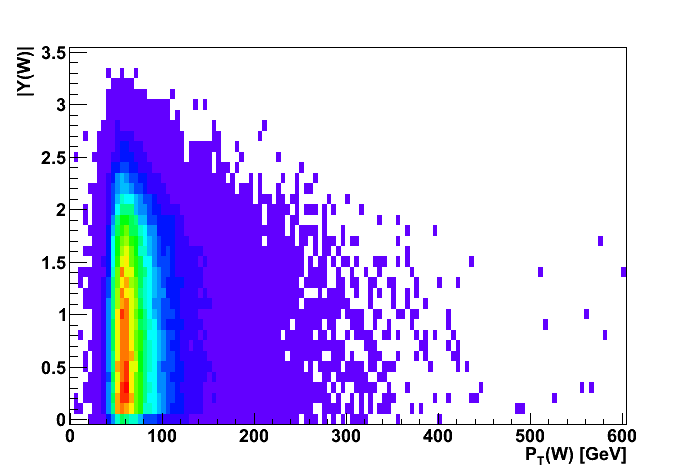
\includegraphics[width=0.45\textwidth]{fig/WPTvsY_mcreco50toinf}}\quad
\subfloat[]{\label{fig:wpol_genreco_ppt}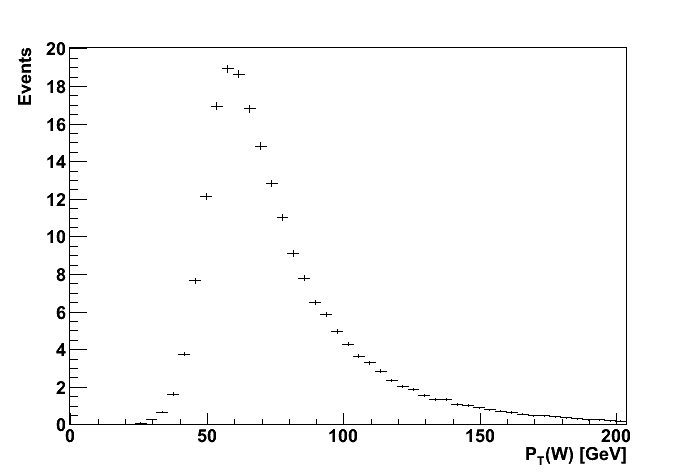
\includegraphics[width=0.45\textwidth]{fig/ptw_mcrecocut}}\quad
\caption{}
\label{fig:wpol_genreco}
\end{figure}

\section{Analysis}
\subsection{Introduction}
To summarise what has already been said, the goal of this analysis is to extract
the helicity fractions (\fL, \fR and \f0) of the \PW boson and thus establish
the dominant left-handed polarisation effect present in theoretical predictions
at high \PtW. The $f_i$ coefficients determine the polar angle distribution
(\thetastar) via Eqn~\ref{eqn:wpol_helicity_fractions}. This distribution cannot
be reconstructed directly due to an ambiguity in the reconstruction of the \PW
boson rest frame. Instead the \LP variable, found to be highly correlated with
$\cos\thetastar$ in the limit of large \PtW is taken instead. Via a reweighting
method, \LP distributions are constructed from Monte-Carlo simulation
corresponding to 100\% left-handed, right-handed and longitudinally polarised
\PW bosons. These shapes may then be used in a fit to data in order to extract
the helicity fractions themselves.

In order to perform this analysis, it is vital that a highly pure sample of \PW
bosons is collected. Additional background contamination must be accounted for
in the fitting procedure, either by subtraction or by incorporation of an
appropriate shape template. However this is handled, it will inevitably
introduce additional uncertainty into the fit. In the case of subtraction,
uncertainty on the shape and normalisation must be accounted for and propagated
into the total uncertainties on the helicity fractions. Introducing an
appropriate template into the fit adds an additional parameter to account for
the relative normalisation as well as uncertainties stemming from the template
shape. This is particularly problematic in the case of \ac{QCD} multijet events
where the underlying processes are felt to be poorly understood. This
necessitates the use of a data-driven template which, as will be seen, brings an
additional set of difficulties.

We shall now motivate and describe each analysis cut for both the muon and
electron channels of the analysis. Due to the differences in the detector
hardware involved, the object selection criteria will of course be different
between the two channels. However, the differing background levels and
composition have necessitated further divergence which will be noted
explicitly. Although both channels will be described in detail, the electrons
will naturally receive more attention, being the focus of the present author's
work.

\subsection{Leptons}
The first selection requirement is to choose events with a charged lepton
consistent with that of a \PW decay. Such events should, at a minimum, contain
at least one reconstructed electron or muon. Wherever possible, the lepton
selection criteria adopted were those used for the \PW cross section analysis
\cite{cms_w_paper}. These requirements had been chosen to be as robust as
possible during the period of early data-taking at \ac{CMS}.

\subsubsection{Muons}
The requirements placed on the muon are as follows:
\begin{itemize}
\item The muon is required to be reconstructed as both a global muon and a
  tracker muon. This is to guard against either global muons mismatched with the
  tracker or noisy muon chambers in the case of tracker muons. For further
  information on muon identification, see Section~TODO.
\item More than 10 hits in the tracker.
\item Bad muon fits are rejected by requiring $\chi^2 < 10$ on the global muon
  fit (tracker and muon chambers)
\item The transverse impact parameter of the muon with respect ot the beamspot
  is required to be $ < \unit{2}{\milli\metre}$. This is a fairly loose
  requirement but still rejects the majority of cosmic muons.
\item At least 1 hit is required in the pixels of the tracker in order to remove
  in-flight decays.
\item The tracker muon reconstruction must involve at least 2 muon stations. This supresses
  punch-through and accidental matchings and ensures compatibility with the
  trigger.
\item The global muon reconstruction must involve at least 1 valid hit in the
  muon chambers; again to guard against decays in flight and punch-through.
\item A cut on the muon pseudorapidity $|\eta| < 2.1$ in order to ensure
  compatibility with the trigger requirements.
\item A cut on the combined isolation,
\begin{equation}
\CombIso = \frac{\sum_{\textrm{tracks}} p_T^{\textrm{track}} + \sum_{\textrm{dep}}
  E_T^{\textrm{had}} + \sum_{\textrm{dep}} E_T^{\textrm{had}}}{\Ptmu}
\end{equation}
where the sums run over the tracks in the tracker or the energy deposits in the
\ac{ECAL} and \ac{HCAL} within a cone of $\Delta R = \sqrt{(\Delta\eta)^2 +
  (\Delta\phi)^2} < 0.3$. A threshold of \unit{0.7}{\GeV} was placed on the
tracks contributing to the isolation sum.
\end{itemize}
Muons passing this set of selection criteria will be referred to as
\textbf{Tight}. Global muons failing one or more of these criteria will be
referred to as \textbf{Loose}.

\subsubsection{Electrons}
Electrons are inheriently less cleanly reconstructed objects than muons. The
object selection is correspondingly more complex to ensure an optimal trade-off
between the efficiency and the purity of the selection. We shall first present
the variables used in the selection.

\begin{itemize}
\item \sigmaieta is a measure of the \ac{RMS} shower width of the electron
  in the $\eta$ direction.
\item \deltaphiin and \deltaetain represent the angular separation between the
  trajectory of the \ac{GSF} track and the ac{ECAL} supercluster.
\item Tracker, \ac{ECAL} and \ac{HCAL} isolation quantities summed in a cone
  $\Delta R < 0.3$. Within the tracker, a threshold of \unit{700}{\GeV} is
  applied to the tracks contributing to the sum. Similarly, in the ac{ECAL}, a
  zero-supression cut is applied. The cone is centred on the track direction at
  the vertex for the tracker isolation, and the supercluster for the calorimeter
  quantities.
\item \HoverE is the ratio of the energy deposited in the \ac{HCAL} behind the
  electron seed to that in the \ac{ECAL}.
\item The track associated with the electron is required to have a hit in the
  first layer of the pixel tracker in order to reject photon conversions.
\item Further rejection against electron conversions is provided by the
  variables \Dist and \DeltaCotTheta. These are calculated by searching for a
  conversion partner of the electron \ac{GSF} track. If such a partner is found,
  the electron is rejected if both \Dist and \DeltaCotTheta are below given thresholds.
\end{itemize}

As part of the \PW cross-section measurement, a number of ``working points''
were defined corresponding to different electron selection efficiencies. A set
of cut values placed on the identification variables just described are then
associated with each working point. These have been chosen via an optimisation
procedure and are further specialised for electrons reconstructed in the barrel
and endcap region. This is to account for the different reconstruction
characteristics in these regions of the detector (see Section~TODO).
% TODO more detail on ID. Possibly should be in object reconstruction chapter.

In order to achieve a strong supression of the \ac{QCD} multi-jet background,
the decision was made to choose a tighter working point than other \ac{CMS}
analyses - the 70\% efficiency working point. Electrons passing these criteria
will be referred to as \textbf{Tight}. For the purposes of vetoing dilepton
events, the 95\% efficiency cuts were used. These will be referred to as
\textbf{Loose} electrons.
% TODO more detail on the choice of the 70\% working point. Perhaps should be
% added later on.

\subsection{Jets}
\label{sec:wpol_jets}
In order to reject events coming from \ttbar decays, which tend to have a large
jet multiplicity, an upper limit is placed on the number of jets in the
event. The jets are clustered using the \antikT algorithm from particle flow
reconstructed objects. A cone radius of 0.5 is used and an acceptance cut
$\modeta < 5$ is applied. Additionally, cleaning is applied to remove jets from
the event within a cone of $\Delta R < 0.3$ of the highest \Pt electron. Such
objects are understood to be an overlap in the reconstruction algorithms. This
could also be addressed by consistent use of particle flow objects for both
electrons and jets.

\subsection{Kinematic Cuts}
\subsubsection{Transverse \PW Momentum}
The most vital kinematic cut to the analysis is the cut on the transverse
momentum of the \PW, \PtW. As has been discussed, requiring \PW bosons with a
large transverse momentum serves to enhance the polarisation effect described in
Section~\ref{sec:polarisation}. It also ensures the correlation of \LP with
$\cos\thetastar$ and thus improves the measurement of the helicity
fractions. There are several means of reconstructing the \PtW at \ac{CMS}. The
first, which was initially used for this analyis was the hadronic recoil of the
event. This is effectively the so-called missing hadronic energy of the
event, or \MHT,
% TODO Perhaps this should be moved somewhere else?
\begin{equation}
\PtW^{\textrm{had}} = - \sum_{j \in \textrm{jets}} \vec{j}
\end{equation}
where the $j$ is taken to run over some subset of the jets in the event as
defined in Section~\ref{sec:wpol_jets} with some minimum transverse momentum
requirement. The sum is taken to denote a vectorial sum. Since the \PW and the
jets must balance in the lab frame, this in principal provides an accurate
measurement of \PtW. However, the reconstruction fo the jets is difficult and
subject to uncertainties in the jet energy scale. A higher resolution
measurement can be achieved by utilising instead the \MET (effectively the
neutrino) and the lepton in the event. This leads to the definition,
\begin{equation}
\PtW^{\textrm{lep}} = \vec{\Pl} + \vec{\MET}
\end{equation}
This provides a higher resolution measurement of \PtW, as can be seen in
Figure~TODO. It is thus the variable adopted in this analysis.

A second question, is then the choice of the minimum cut value to place on
\PtW. On the one hand, increasing this cuts reduces the statistics of the
sample. A related difficulty for this analysis was the small size of the
simulated $\PW\longrightarrow\Pl\Pgn$ sample, particularly at higher \PtW. On
the other hand, the enhancment of the polarisation effect and the increased
correlation between $\cos\thetastar$ motivate a larger cut value. The benefits of
these two effects could also be gained by binning the sample in \PtW and
performing independent fits within each bin. Unfortunately, the data sample
available had inadequate statistics to make such an approach feasible. Instead,
a moderately large $\PtW > \unit{50}{\GeV}$ was adopted.
% TODO mroe detail on this choice!




%%% Local Variables:
%%% mode: latex
%%% TeX-master: "../thesis"
%%% End:
